% This file was created by tikzplotlib v0.9.2.
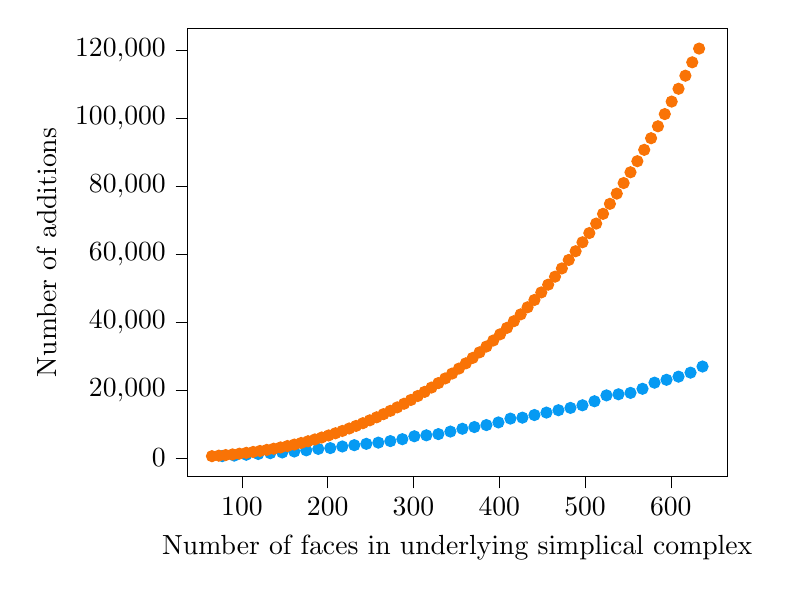
\begin{tikzpicture}
\definecolor{color0}{rgb}{0.0235294117647059,0.603921568627451,0.952941176470588}
\definecolor{color1}{rgb}{0.976470588235294,0.450980392156863,0.0235294117647059}

\begin{axis}[
xlabel = Number of faces in underlying simplical complex,
tick align=outside,
tick pos=left,
x grid style={white!69.0196078431373!black},
xmin=36.4, xmax=665.6,
xtick style={color=black},
ylabel = Number of additions,
y grid style={white!69.0196078431373!black},
ymin=-5447.05, ymax=126620.05,
ytick style={color=black},
yticklabel style={
        /pgf/number format/fixed,
        /pgf/number format/precision=5
},
scaled y ticks=false
]
\addplot [only marks, mark=*, draw=color0, fill=color0, colormap/viridis]
table{%
x                      y
77 569
91 723
105 980
119 1203
133 1439
147 1651
161 1930
175 2273
189 2694
203 2931
217 3408
231 3792
245 4184
259 4544
273 4994
287 5559
301 6417
315 6696
329 7053
343 7798
357 8627
371 9133
385 9713
399 10495
413 11620
427 11901
441 12674
455 13391
469 14095
483 14775
497 15544
511 16727
525 18461
539 18782
553 19196
567 20405
581 22205
595 23053
609 23980
623 25158
637 26965
};
\addplot [only marks, mark=*, draw=color1, fill=color1, colormap/viridis]
table{%
x                      y
65 556
73 707
81 879
89 1073
97 1290
105 1531
113 1797
121 2089
129 2408
137 2755
145 3131
153 3537
161 3974
169 4443
177 4945
185 5481
193 6052
201 6659
209 7303
217 7985
225 8706
233 9467
241 10269
249 11113
257 12000
265 12931
273 13907
281 14929
289 15998
297 17115
305 18281
313 19497
321 20764
329 22083
337 23455
345 24881
353 26362
361 27899
369 29493
377 31145
385 32856
393 34627
401 36459
409 38353
417 40310
425 42331
433 44417
441 46569
449 48788
457 51075
465 53431
473 55857
481 58354
489 60923
497 63565
505 66281
513 69072
521 71939
529 74883
537 77905
545 81006
553 84187
561 87449
569 90793
577 94220
585 97731
593 101327
601 105009
609 108778
617 112635
625 116581
633 120617
};
\end{axis}

\end{tikzpicture}
